\documentclass[Serif, 10pt, brown]{beamer}
\usepackage{booktabs,xcolor}
\usepackage{pifont}
\newcommand*\CHECK{\ding{51}}
\usepackage{array}
\newcolumntype{P}[1]{>{\centering\arraybackslash}p{#1}}

\usepackage{setspace,mathtools,amssymb,multirow,array,amsmath,tikz}
\usepackage[normalsize]{subfigure}
\usetikzlibrary{patterns,automata,positioning,decorations.pathreplacing,decorations,calc}
\usepackage{curves}
\usepackage{caption}
\usepackage{wasysym}
\usepackage{epsfig,epstopdf,graphicx}

\curvewarnfalse

\newtheorem{proposition}{Proposition}
\theoremstyle{example}
\newtheorem{theoremh}{Theorem}
\theoremstyle{plain}
\renewcommand{\textfraction}{0.01}
\renewcommand{\floatpagefraction}{0.99}
\newcommand{\ul}{\underline}
\newcounter{units}
\setbeamercovered{dynamic}
\logo{\includegraphics[width=0.5in,keepaspectratio]{\FIGDIR/iitb_logo.png}}
\newcommand{\FIGDIR}{../figures} 
\newcommand{\RESULTDIR}{../../results} 
\mode<presentation>{
    \usetheme[right,currentsection,hideothersubsections]{UTD}
    \useoutertheme{sidebar}
    \useinnertheme[shadow]{rounded}
    \usecolortheme{whale}
    \usecolortheme{orchid}
    \usefonttheme[onlymath]{serif}
    \setbeamertemplate{footline}{\centerline{Slide \insertframenumber/\inserttotalframenumber}}
}

\usebeamercolor[fg]{author in sidebar}
\title[{Systems for LLMs}]{\sc Benchmarking and Performance Analysis of LLM Inferencing Systems}
\author[\ul{Saksham Rathi}]{{\textbf{Saksham Rathi}}}
\institute[UTD]{\sc\small Systems for LLMs\\ Under Prof. Mythili Vutukuru}
\date[UCI]{Indian Institute of Technology Bombay \\ Autumn 2025-26}

\begin{document}
\frame{\titlepage}

\begin{frame}{Contents}
	\tableofcontents
\end{frame}

\section{Various Scheduler Designs}
\subsection{vLLM Schedulers}
\begin{frame}{First Come First Serve Policy}
    \begin{itemize}
        \item Adds requests one by one, from the core engine into a waiting queue
        \item The requests are extracted in a first come first serve manner
        \item We stop selecting requests from the waiting queue into the running batch, once the size reaches \texttt{max\_batch\_size}
    \end{itemize}
\end{frame}

\begin{frame}{Priority Based}
    \begin{itemize}
        \item The user passes priority values along with the requests' strings themselves
        \item We use a min heap to find the request with the smallest priority value (executed at first)
        \item Ties are broken in a first come first serve manner (through tracking request's arrival time)
    \end{itemize}
\end{frame}

\subsection{Our Schedulers}
\begin{frame}{Greedy First Come First Serve}
    \begin{itemize}
        \item We keep a track of the working set along with the requests we add to the current running scheduler batch
        \item We add requests in a first come first serve manner
        \item However, now we are also controlling the batch size - we stop whenever addition of the next request increases the working set size beyond a threshold (decided by L2 cache size)
        \item For our workload, and GPU - it boils down to stopping whenever the next request belongs to a different family
    \end{itemize}
\end{frame}

\begin{frame}{Greedy First Come First Serve - Appendix - Expected Batch Size}
    Let's say we have $N$ families. The user passes a bunch of requests, which can belong to any of these families. Moreover, all the requests have been shuffled, such that the probability of a request at position $i$ to be of family $j$ is exactly $\frac{1}{N}$.

    Assume that the first request belongs to family $j$. We find out the expected value of the size of the first scheduler batch.

    For the batch to have size exactly $x$:
    \begin{itemize}
        \item The first $x - 1$ requests after the initial one must also be of family $j$.
        \item The $x$-th request must be of a different family.
    \end{itemize}


    The probability that the batch is of size $x$ is given by:
    \[
        \Pr[X = x]
        = \left(\frac{1}{N}\right)^{x-1} \cdot \frac{N-1}{N}, \quad x \ge 1.
    \]
\end{frame}



\begin{frame}{Greedy First Come First Serve - Appendix - Expected Batch Size}
    Let $X$ denote the size of the first batch. Its expected value is:
    \[
        \mathbb{E}[X]
        = \sum_{x=1}^{\infty} x \Pr[X = x]
        = \sum_{x=1}^{\infty} x \left(\frac{1}{N}\right)^{x-1} \frac{N-1}{N}.
    \]
    Using the identity
    \[
        \sum_{x=1}^{\infty} x r^{x-1} = \frac{1}{(1-r)^2}, \quad |r| < 1,
    \]
    with $r = \frac{1}{N}$, we obtain:
    \[
        \mathbb{E}[X]
        = \frac{N-1}{N} \cdot \frac{1}{\left(1 - \frac{1}{N}\right)^2}
        = \frac{N}{N-1}.
    \]

    \vspace{0.3cm}
    \[
        \boxed{\mathbb{E}[\text{batch size}] = \frac{N}{N-1}}
    \]

    For example, when we have 2 families, the expected batch size would be just 2.
\end{frame}


\begin{frame}{Family ID Based}
    \begin{itemize}
        \item If we can set priority values for each of the request, then why can't we set the family to which they belong to?
        \item We have separate queues for each family
        \item All the individual queues operate in a first come first serve manner
        \item If there is a request of family ID $j$ already present in the scheduler batch, then we try to add all the requests of that family in the same batch (till we hit \texttt{max\_batch\_size}). If there is no request of that family available, then we stick to the current batch (no more requests added)
        \item So, the batch size is no longer static - it is dynamically set in accordance with the workload
    \end{itemize}
\end{frame}

\begin{frame}{Radix Tree Based}
    \begin{itemize}
        \item Key idea: Instead of treating each request independently, we exploit shared token prefixes across requests
        \item Each request is represented as a path of tokens in a radix tree
        \item Internal nodes correspond to shared token substrings 
        \item The scheduler maintains a working set of active nodes (tokens already materialized / cached)
        \item Each waiting request has a cost = number of tokens missing from the working set
    \end{itemize}
\end{frame}

\begin{frame}{Radix Tree Based}
    To schedule the next request:
    \begin{itemize}
        \item We start from leaves already in the working set
        \item Traverse upwards toward the root
        \item At each node, we look for waiting requests passing through it
        \item We select the request with minimum missing-token cost
    \end{itemize}
    Activating a request:
    \begin{itemize}
        \item Adds its path to the working set
        \item Future requests that share prefixes become cheaper
        \item This dynamically forms prefix-coherent batches, minimizing recomputation
    \end{itemize}
\end{frame}


\begin{frame}{Radix Tree Based - Radix Tree Construction}
\centering
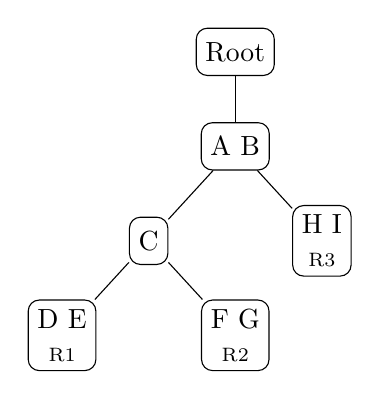
\begin{tikzpicture}[
    every node/.style={draw, rectangle, rounded corners, minimum height=6mm, align=center},
    level distance=12mm,
    sibling distance=22mm
]

\node {Root}
    child {
        node {A B}
        child {
            node {C}
            child {
                node {D E\\{\scriptsize R1}}
            }
            child {
                node {F G\\{\scriptsize R2}}
            }
        }
        child {
            node {H I\\{\scriptsize R3}}
        }
    };

\end{tikzpicture}

\vspace{1em}
\small
Each leaf corresponds to a request.  
Internal nodes represent shared token prefixes.
\end{frame}

\begin{frame}{Radix Tree Based - Working Set After Activation}
\centering
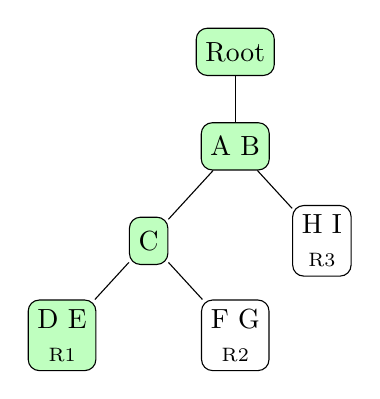
\begin{tikzpicture}[
    every node/.style={draw, rectangle, rounded corners, minimum height=6mm, align=center},
    ws/.style={fill=green!25},
    level distance=12mm,
    sibling distance=22mm
]

\node[ws] {Root}
    child {
        node[ws] {A B}
        child {
            node[ws] {C}
            child {
                node[ws] {D E\\{\scriptsize R1}}
            }
            child {
                node {F G\\{\scriptsize R2}}
            }
        }
        child {
            node {H I\\{\scriptsize R3}}
        }
    };

\end{tikzpicture}

\vspace{1em}
\small
Green nodes indicate the working set after activating R1.
\end{frame}

\begin{frame}{Radix Tree Based - Finding the Best Request}
\centering
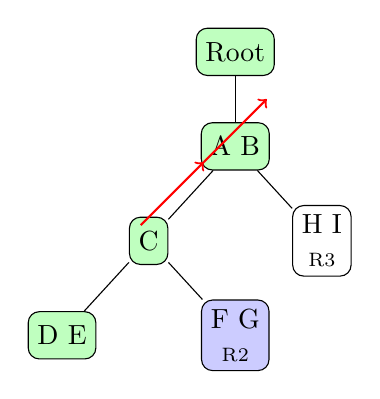
\begin{tikzpicture}[
    every node/.style={draw, rectangle, rounded corners, minimum height=6mm, align=center},
    ws/.style={fill=green!25},
    candidate/.style={fill=blue!20},
    level distance=12mm,
    sibling distance=22mm
]

\node[ws] {Root}
    child {
        node[ws] {A B}
        child {
            node[ws] {C}
            child {
                node[ws] {D E}
            }
            child {
                node[candidate] {F G\\{\scriptsize R2}}
            }
        }
        child {
            node {H I\\{\scriptsize R3}}
        }
    };

\draw[->, thick, red] (-1.2,-2.2) -- (-0.4,-1.4);
\draw[->, thick, red] (-0.4,-1.4) -- (0.4,-0.6);

\end{tikzpicture}

\vspace{1em}
\small
Traversal starts from working-set leaves and moves upward.  
R2 is selected due to maximum prefix overlap.
\end{frame}


\begin{frame}{Radix Tree Based - Dynamic Batch Growth}
\centering
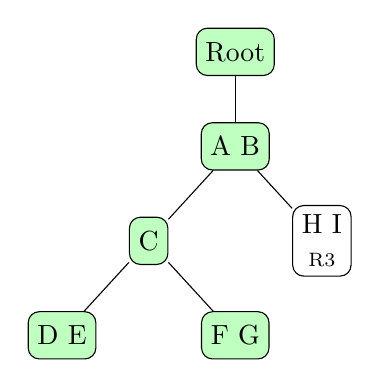
\begin{tikzpicture}[
    every node/.style={draw, rectangle, rounded corners, minimum height=6mm, align=center},
    ws/.style={fill=green!25},
    level distance=12mm,
    sibling distance=22mm
]

\node[ws] {Root}
    child {
        node[ws] {A B}
        child {
            node[ws] {C}
            child {
                node[ws] {D E}
            }
            child {
                node[ws] {F G}
            }
        }
        child {
            node {H I\\{\scriptsize R3}}
        }
    };

\end{tikzpicture}

\vspace{1em}
\small
Batch size grows dynamically as long as marginal cost is low.
\end{frame}

\begin{frame}{Radix Tree Based - Issues}
    The above approach has a few issues:
    \begin{itemize}
        \item Adding a request is quite costly - there might be splitting/merging of nodes. Although finding the best request is quite efficient
        \item Each request may contain thousands of tokens, so the tree depth might get quite large too
        \item We cannot have a parallel thread/process handling the radix tree, because maintaining sync is difficult. What if we removed a request, from our waiting queue, but it takes some time to remove it from the radix tree?
    \end{itemize}
\end{frame}

\begin{frame}{Chunked Hash Tree Based}
\begin{itemize}
    \item Requests are represented using \textbf{hashed cumulative prefixes}
    \item Tokens are divided into fixed-size chunks
    \item Each level corresponds to \texttt{hash(tokens[0:k])}
    \item No explicit tree structure or node splitting
    \item Much faster than radix trees for large workloads
\end{itemize}
\end{frame}

\begin{frame}{Chunked Hash Tree Based - Working Set}
\begin{itemize}
    \item Working set = set of active \textbf{(level, hash)} pairs
    \item Each active request contributes all its prefix hashes
    \item Request cost = number of missing prefix hashes
    \item Scheduling prefers requests with minimal missing chunks
    \item Enables dynamic batch growth similar to radix trees
\end{itemize}
\end{frame}

\begin{frame}{Chunked Hash Tree Based - Insertion}
\centering
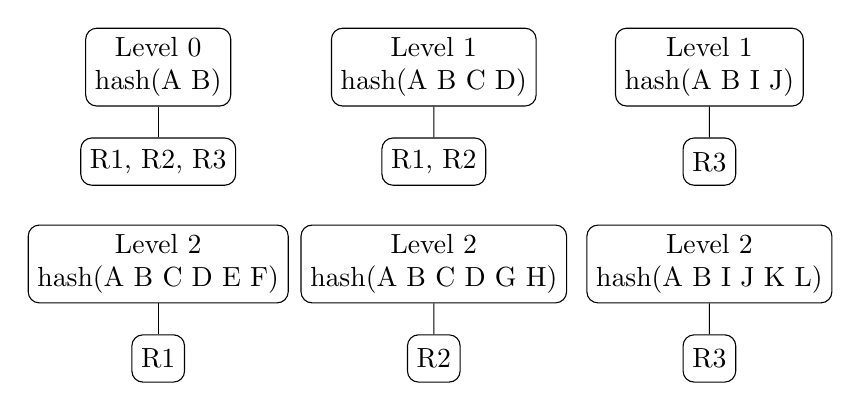
\begin{tikzpicture}[
    every node/.style={draw, rectangle, rounded corners, minimum height=6mm, align=center},
    level distance=12mm,
    sibling distance=32mm
]
\node (level0) at (0,0) {Level 0\\hash(A B)}
    child { node {R1, R2, R3} };
\node (level1) at (3.5,0) {Level 1\\hash(A B C D)}
    child { node {R1, R2} };
\node (level1) at (7,0) {Level 1\\hash(A B I J)}
    child { node {R3} };
\node at (0,-2.5) {Level 2\\hash(A B C D E F)}
    child { node {R1} };
\node at (3.5,-2.5) {Level 2\\hash(A B C D G H)}
    child { node {R2} };
\node at (7,-2.5) {Level 2\\hash(A B I J K L)}
    child { node {R3} };
\end{tikzpicture}
\vspace{0.5em}
\small
Each level stores hashes of cumulative token prefixes.
\end{frame}

\begin{frame}{Chunked Hash Tree Based - Working Set}
\centering
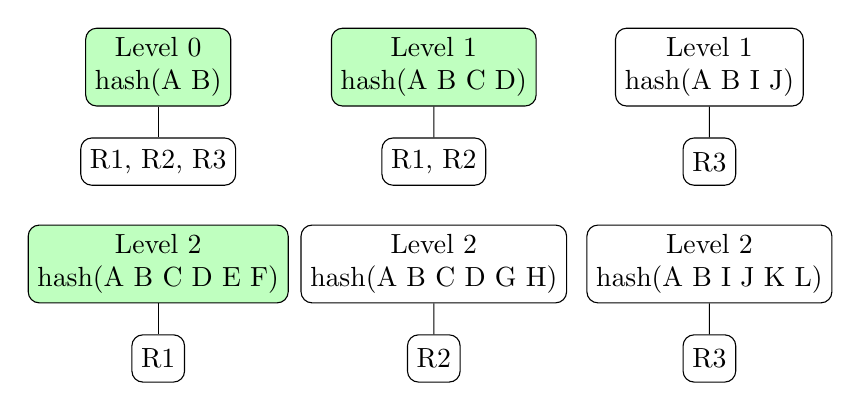
\begin{tikzpicture}[
    every node/.style={draw, rectangle, rounded corners, minimum height=6mm, align=center},
    ws/.style={fill=green!25},
    level distance=12mm,
    sibling distance=32mm
]
\node[ws] (level0) at (0,0) {Level 0\\hash(A B)}
    child { node {R1, R2, R3} };
\node[ws] (level1) at (3.5,0) {Level 1\\hash(A B C D)}
    child { node {R1, R2} };
\node (level1) at (7,0) {Level 1\\hash(A B I J)}
    child { node {R3} };
\node[ws] at (0,-2.5) {Level 2\\hash(A B C D E F)}
    child { node {R1} };
\node at (3.5,-2.5) {Level 2\\hash(A B C D G H)}
    child { node {R2} };
\node at (7,-2.5) {Level 2\\hash(A B I J K L)}
    child { node {R3} };
\end{tikzpicture}
\vspace{0.5em}
\small
Green boxes indicate prefix hashes in the working set.
\end{frame}

\begin{frame}{Chunked Hash Tree Based - Best Request Selection}
\centering
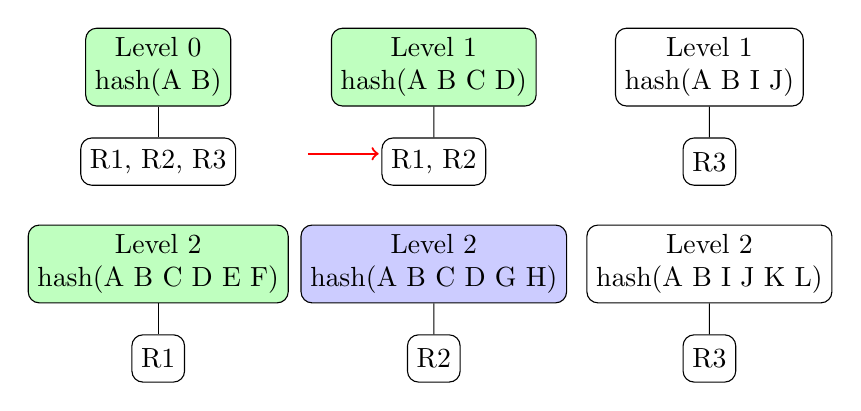
\begin{tikzpicture}[
    every node/.style={draw, rectangle, rounded corners, minimum height=6mm, align=center},
    ws/.style={fill=green!25},
    candidate/.style={fill=blue!20},
    level distance=12mm,
    sibling distance=32mm
]
\node[ws] (level0) at (0,0) {Level 0\\hash(A B)}
    child { node {R1, R2, R3} };
\node[ws] (level1) at (3.5,0) {Level 1\\hash(A B C D)}
    child { node {R1, R2} };
\node (level1) at (7,0) {Level 1\\hash(A B I J)}
    child { node {R3} };
\node[ws] at (0,-2.5) {Level 2\\hash(A B C D E F)}
    child { node {R1} };
\node[candidate] at (3.5,-2.5) {Level 2\\hash(A B C D G H)}
    child { node {R2} };
\node at (7,-2.5) {Level 2\\hash(A B I J K L)}
    child { node {R3} };
\draw[->, thick, red] (1.9,-1.1) -- (2.8,-1.1);
\end{tikzpicture}
\vspace{0.5em}
\small
Green boxes indicate prefix hashes in the working set. 

R2 is selected since it has maximum prefix overlap with the working set.
\end{frame}

\subsection{Already Existing Schedulers}

\begin{frame}{Dynamic Batching}
    \begin{itemize}
        \item Static batching uses a fixed maximum batch size
        \item Dynamic batching adapts batch size based on \textbf{runtime GPU memory state}
        \item Memory usage is dominated by KV cache allocation
        \item Larger batches improve throughput but increase memory pressure
    \end{itemize}
\end{frame}

\begin{frame}{Dynamic Batching - Memory-Aware Control}
    \begin{itemize}
        \item Let $B$ be the current batch size
        \item Measure used GPU blocks and estimate blocks per sequence:
        \[
            \text{blocks\_per\_seq} = \frac{\text{used GPU blocks}}{B}
        \]
        \item Compute the memory-safe maximum batch size:
        \[
            B_{\max} =
            \left\lfloor
            \frac{\text{total GPU blocks} \times \alpha}
                 {\text{blocks\_per\_seq}}
            \right\rfloor
        \]
        \item $\alpha$ is a safety factor (e.g., $\alpha = 0.95$)
        \item Stop adding requests when $B \ge B_{\max}$
    \end{itemize}
\end{frame}



\begin{frame}{BucketServe - Bucket-Based Dynamic Batching}
    \begin{itemize}
        \item Real-world workloads exhibit \textbf{highly heterogeneous sequence lengths}
        \item Naive batching mixes short and long requests, causing:
        \begin{itemize}
            \item Excessive padding
            \item GPU memory waste
            \item Lower effective throughput
        \end{itemize}
        \item Key idea: \textbf{group requests by sequence length} before batching
        \item Enables tighter memory bounds and more predictable batch sizing
    \end{itemize}
\end{frame}

\begin{frame}{BucketServe: Design}
    \begin{itemize}
        \item Incoming requests are assigned to \textbf{length-homogeneous buckets}
        \item Each bucket covers a sequence length interval:
        \[
            [L_b, U_b)
        \]
        \item Buckets reduce padding by minimizing ($S$ is the sequence length):
        \[
            S_{\max} - S_{\mathrm{avg}}
        \]
        \item Dynamic batching is applied \textbf{within each bucket}
        \item Batch size is adjusted based on:
        \begin{itemize}
            \item GPU memory availability
            \item Maximum sequence length in the bucket
        \end{itemize}
    \end{itemize}
\end{frame}
\begin{frame}{BucketServe : Memory Safety}
    \begin{itemize}
        \item Bucket boundaries are adjusted online based on workload distribution
        \item Buckets are:
        \begin{itemize}
            \item \textbf{Split} when length variance is high
            \item \textbf{Merged} under low load to reduce scheduling overhead
        \end{itemize}
        \item For each bucket, compute a memory-safe batch size:
        \[
            N_{\max} =
            \max \left\{
            N \;\middle|\;
            \sum_{i=1}^{N} S_i \le M_{\text{safe}}
            \right\}
        \]
        \item Not too relevant for our workload, because the query sizes are roughly similar, and system prompt is anyway shared, so the expected throughput is quite similar to that of vLLM baseline
    \end{itemize}
\end{frame}

\subsection{SGLANG Schedulers}
\begin{frame}{LPM: Longest Prefix Matching}
    \begin{itemize}
        \item Prioritizes requests based on how much of their input prefix already exists in the prefix cache
        \item Requests with longer cached prefixes are scheduled earlier
        \item If multiple requests share a short prefix that is not yet cached, only a few are scheduled first. Others may be temporarily deprioritized to allow one request to populate the cache
        \item If the waiting queue is large (e.g., $>$ 128 requests), LPM is disabled and falls back to FCFS to avoid expensive prefix matching
    \end{itemize}
\end{frame}

\begin{frame}{DFS Weight}
    \begin{itemize}
        \item Organizes requests according to the structure of the prefix cache tree
        \item Each request is associated with a last matched node in the prefix tree
        \item Each tree node is assigned a weight equal to the number of requests ending at that node plus the weights of all its descendant nodes
        \item Perform DFS: add requests in that order (visit children in descending order of weights)
    \end{itemize}
\end{frame}

\section{Throughput Numbers}
\begin{frame}{Workload Setup}
    \begin{itemize}
        \item Two families (each of system prompt of length 1300 tokens)
        \item 2500 queries of each family - total 5000 queries
        \item All randomly shuffled
        \item L2 Cache size = 96 MB (RTX 6000 Ada Generation)
        \item Each family's system prompt's KVCache roughly takes 180 MB (model: Llama3.1-8B)
        \item We measure end-to-end throughput (including the time taken to add/process requests)
        \item We generate 50 new tokens for each request
    \end{itemize} 
\end{frame}

\begin{frame}{Why just 50 new tokens?}
    \begin{itemize}
        \item LLMs hardly answer in 1-2 sentences, so less than 50 (like somewhere around 10-20) does not make much sense
        \item The scheduler changes help increasing L2 purity, even during decodes, so larger number of output tokens show better throughput improvement
        \item Having 200 new tokens for a shared prefix of length 1300 tokens reduces the amount of overlap between two queries
    \end{itemize}
\end{frame}

\begin{frame}{Throughput}
\begin{table}[h!]
\centering
\scriptsize
\begin{tabular}{|p{2.5cm}|c|p{4cm}|}
\hline
\textbf{Scheduler} & \textbf{Throughput (req/sec)} & \textbf{Comments} \\
\hline
    First Come First Serve & 45.49 & vLLM Baseline \\
    First Come First Serve - Family Ordered & 64.97 & User orders the requests by their families ; theoretical maximum which a user can get from vLLM through client side changes \\
    Greedy First Come First Serve & 2.04 & Due to very small batch size \\
    Family ID Based & 86.72 & The fastest which we can achieve ; although through demanding additional information from the user \\
    Radix Tree Based & 53.06 & Inefficient design ; too much CPU overhead ; consumes a lot of time in between scheduler iterations \\
    Chunked Hash Tree Based & 77.44 & A much more efficient design ; quite less overhead ; no extra information needed from the user \\
    Dynamic Batching & 46.98 & Max batch size set to 1000 \\
\hline
\end{tabular}
\caption{Throughput Across Different Scheduler Designs}
\end{table}

\end{frame}


\begin{frame}{Throughput (for max new tokens = 100)}
\begin{table}[h!]
\centering
\scriptsize
\begin{tabular}{|c|c|}
\hline
\textbf{Scheduler} & \textbf{Throughput (req/sec)} \\
\hline
    First Come First Serve & 20.84 \\
    First Come First Serve - Family Ordered & 33.94 \\
    Family ID Based & 42.73  \\
    Chunked Hash Tree Based & 43.20  \\
\hline
\end{tabular}
\caption{Throughput Across Different Scheduler Designs}
\end{table}

\end{frame}


\begin{frame}{Throughput (for max new tokens = 200)}
\begin{table}[h!]
\centering
\scriptsize
\begin{tabular}{|c|c|}
\hline
\textbf{Scheduler} & \textbf{Throughput (req/sec)} \\
\hline
    First Come First Serve & 10.67 \\
    First Come First Serve - Family Ordered & 18.78 \\
    Family ID Based & 21.14 \\
    Chunked Hash Tree Based & 21.34  \\
\hline
\end{tabular}
\caption{Throughput Across Different Scheduler Designs}
\end{table}

\end{frame}

\begin{frame}{Throughput vs Sequence length}
    \begin{figure}
        \centering
    \includegraphics[width=0.8\textwidth]{\RESULTDIR/throughput_vs_seq_length.png}
    \captionof{figure}{Throughput vs Sequence Length}
\end{figure}
\end{frame}

\begin{frame}{Throughput vs req/sec}
    We model the request ingestion as a poisson process (basically, with exponential sleep times between two consecutive requests)
    \begin{figure}
        \centering
    \includegraphics[width=0.8\textwidth]{\RESULTDIR/throughput_vs_req_per_sec_poisson.png}
    \captionof{figure}{Throughput vs Varying Ingestion}
\end{figure}
\end{frame}

\begin{frame}{Throughput vs Sequence length (vLLM vs SGLANG)}
    \begin{figure}
        \centering
    \includegraphics[width=0.8\textwidth]{\RESULTDIR/throughput_vllm_sglang_comparison_scheduling_policies.png}
    \captionof{figure}{Throughput vs Sequence Length (vLLM vs SGLANG)}
\end{figure}
\end{frame}

\begin{frame}{Throughput vs Req/sec (2 families)}
    \begin{figure}
        \centering
    \includegraphics[width=0.8\textwidth]{\RESULTDIR/throughput_vs_req_sec_families_2_poisson.png}
    \captionof{figure}{Throughput vs Req/sec (2 families)}
    \end{figure}
\end{frame}

\begin{frame}{Throughput vs Req/sec (5 families)}
    \begin{figure}
        \centering
    \includegraphics[width=0.8\textwidth]{\RESULTDIR/throughput_vs_req_sec_families_5_poisson.png}
    \captionof{figure}{Throughput vs Req/sec (5 families)}
    \end{figure}
\end{frame}

\begin{frame}{Throughput vs Req/sec (10 families)}
    \begin{figure}
        \centering
    \includegraphics[width=0.8\textwidth]{\RESULTDIR/throughput_vs_req_sec_families_10_poisson.png}
    \captionof{figure}{Throughput vs Req/sec (10 families)}
    \end{figure}
\end{frame}

\begin{frame}{Throughput vs Req/sec (20 families)}
    \begin{figure}
        \centering
    \includegraphics[width=0.8\textwidth]{\RESULTDIR/throughput_vs_req_sec_families_20_poisson.png}
    \captionof{figure}{Throughput vs Req/sec (20 families)}
    \end{figure}
\end{frame}


\begin{frame}{DRAM Metric}
    \begin{figure}
        \centering
    \includegraphics[width=\textwidth]{\RESULTDIR/dram_meaning.png}
    \captionof{figure}{DRAM Accesses' Metric (from DCGMI)}
    \end{figure}
\end{frame}

\begin{frame}{DRAM Accesses' CDF}
    \begin{figure}
        \centering
    \includegraphics[width=0.7\textwidth]{\RESULTDIR/drama_family_fcfs.png}
    \captionof{figure}{DRAM Accesses' CDF (2 families, 6500 tokens shared context, throughput gain was roughly 4x, metric sampled every 1ms)}
    \end{figure}
\end{frame}

\begin{frame}{DRAM Accesses' Statistics}
    \begin{figure}
        \centering
    \includegraphics[width=0.5\textwidth]{\RESULTDIR/dram_stats_10.png}
    \captionof{figure}{DRAM Accesses' Stats (2 families, 13000 tokens shared context, metric sampled every 1ms)}
    \end{figure}
\end{frame}

\begin{frame}{Batch Decomposition - 200 requests - single family}
    \begin{figure}
        \centering
    \includegraphics[width=0.8\textwidth]{\RESULTDIR/batch_decomposition/200_1_fam.png}
    \captionof{figure}{Decode Stats, 200 requests, single family, 1300 tokens shared context}
    \end{figure}
\end{frame}


\begin{frame}{Batch Decomposition - 200 requests - two families}
    \begin{figure}
        \centering
    \includegraphics[width=0.8\textwidth]{\RESULTDIR/batch_decomposition/200_2_fam.png}
    \captionof{figure}{Decode Stats, 200 requests, two families, 1300 tokens shared context}
    \end{figure}
\end{frame}

\begin{frame}{Batch Decomposition - 500 requests - single family}
    \begin{figure}
        \centering
    \includegraphics[width=0.8\textwidth]{\RESULTDIR/batch_decomposition/500_1_fam.png}
    \captionof{figure}{Decode Stats, 500 requests, single family, 1300 tokens shared context}
    \end{figure}
\end{frame}


\begin{frame}{Batch Decomposition - 500 requests - five families}
    \begin{figure}
        \centering
    \includegraphics[width=0.8\textwidth]{\RESULTDIR/batch_decomposition/500_5_fam.png}
    \captionof{figure}{Decode Stats, 500 requests, five families, 1300 tokens shared context}
    \end{figure}
\end{frame}


\section{Key Propositions}
\begin{frame}{Key Propositions}
    Just to summarize, we have the following key propositions:
    \begin{itemize}
        \item We can operate in a dynamic workload - where requests are being added continuously, unlike BatchLLM
        \item The ChunkedHashTree can work on arbitrarily long requests, with significantly low CPU overhead (can be optimized more)
        \item We know on when to stop, basically if the prefixes change by a huge amount on adding the next request, we will stop adding stuff at that point, even if we didn't hit \texttt{max\_batch\_size} parameter (missing in all the existing approaches, we know of)
        \item Our benefits are based on L2 cache purity, instead of being benefitted from Radix Tree Node LRU Eviction from HBM
    \end{itemize}
\end{frame}


\section{L2Cache Simulator}
\begin{frame}{Simulator Design}
    \begin{itemize}
        \item Software model of L2 cache behaviour during batched LLM inference
        \item Multiple concurrent LLM requests
        \item Accessing KV cache blocks
        \item Over many decode iterations
        \item With/without hardware prefetching
    \end{itemize}
\end{frame}

\begin{frame}{Parameters we can tweak}
    \begin{itemize}
        \item Number of families: 1/2/5
        \item Requests per family: we fix the scheduler batch size to 500, so 500/250/100 requests per family
        \item Blocks per request: vLLM's block stores 16 tokens; assuming a shared context of 6400 tokens: 400 blocks + 1 block for the distinct suffix (query itelf)
        \item Decode iterations: 100
        \item L2 cache size: For our GPU it is 96MB. A shared context of 1300 tokens amounts to 180MB for LLama3.1-8B model. So, 96MB amounts to 44 blocks roughly, out of which we can assume that we have 25 blocks reserved for KV caches (and others for weights/activation tensors etc)
        \item Number of parallel processing units: We have 142 SMs, and each SM has 64 warps, however each attention kernel might use multiple warps, so let us assume 200 parallel processing units
    \end{itemize}
\end{frame}


\begin{frame}{Simulation Flow}
    \begin{itemize}
        \item The simulator runs for a fixed number of decode iterations
        \item In each iteration:
        \begin{enumerate}
            \item All requests are reset to initial state
            \item A batch of requests is scheduled to run in parallel
            \item Each scheduled request generates a sequence of memory accesses
            \item Each access is processed by the L2 cache model
            \item Cache hit/miss statistics are updated
            \item Prefetching is triggered, if enabled
        \end{enumerate}
        \item This loop repeats for 100 decode iterations
    \end{itemize}
\end{frame}


\begin{frame}{L2 Cache Model}
    \begin{itemize}
        \item Modeled as a fixed-size LRU cache
        \item Capacity: 25 KV blocks
        \item For every block access:
        \begin{itemize}
            \item If block is in cache $\rightarrow$ demand hit
            \item If not in cache $\rightarrow$ demand miss + DRAM access
            \item Block is inserted and LRU order updated
        \end{itemize}
        \item Evicted prefetched blocks are counted as wasted
    \end{itemize}
\end{frame}

\begin{frame}{Stride-Based Prefetching}
    \begin{itemize}
        \item Maintains a small history of recent accesses
        \item Computes stride between consecutive blocks (mostly 1)
        \item If the same stride repeats with high confidence:
        \begin{itemize}
            \item Predict future blocks using that stride
            \item Issue prefetches ahead of time
        \end{itemize}
    \end{itemize}
\end{frame}

\begin{frame}{Spatial Region Prefetching}
    \begin{itemize}
        \item Spatial locality in address space
        \item When block $i$ is accessed:
        \begin{itemize}
            \item Also prefetch nearby blocks
            \item $i+1, i+2, ...$ within a small window
        \end{itemize}
        \item Useful when:
        \begin{itemize}
            \item adjacent KV blocks are likely to be reused
            \item access patterns are not perfectly sequential
        \end{itemize}
    \end{itemize}
\end{frame}

\begin{frame}{Simulator stats - 1 family}

\begin{columns}
    \column{0.48\textwidth}
    \centering
    \textbf{Without Prefetching}
    
    \vspace{2mm}
    
    {\scriptsize \begin{tabular}{|l|r|}
        \hline
        Metric & Value \\
        \hline
        Cache Hit Rate & 66.96\% \\
        DRAM Accesses & 6,625,496 \\
        Demand Hits & 13,424,504 \\
        Demand Misses & 6,625,496 \\
        Total Accesses & 20,050,000 \\
        \hline
    \end{tabular}}

    \column{0.48\textwidth}
    \centering
    \textbf{With Prefetching}
    
    \vspace{2mm}
    
    {\scriptsize \begin{tabular}{|l|r|}
        \hline
        Metric & Value \\
        \hline
        Cache Hit Rate & 64.25\% \\
        DRAM Accesses & 22,971,098 \\
        Demand Hits & 12,881,255 \\
        Demand Misses & 7,168,745 \\
        Total Accesses & 20,050,000 \\
        Useful Prefetches & 4,196,846 \\
        Wasted Prefetches & 11,605,500 \\
        Prefetch Accuracy & 26.56\% \\
        Stride Prefetches & 2,172,430 \\
        Region Prefetches & 40,000,000 \\
        Next-Line Prefetches & 0 \\
        \hline
    \end{tabular}}

\end{columns}

\vspace{3mm}

\centering
\small

\end{frame}

\begin{frame}{Simulator Stats - 5 families}

\begin{columns}
    \column{0.48\textwidth}
    \centering
    \textbf{Without Prefetching}
    
    \vspace{2mm}
    
    {\scriptsize \begin{tabular}{|l|r|}
        \hline
        Metric & Value \\
        \hline
        Cache Hit Rate & 15.08\% \\
        DRAM Accesses & 17,027,080 \\
        Demand Hits & 3,022,920 \\
        Demand Misses & 17,027,080 \\
        Total Accesses & 20,050,000 \\
        \hline
    \end{tabular}}

    \column{0.48\textwidth}
    \centering
    \textbf{With Prefetching}
    
    \vspace{2mm}
    
    {\scriptsize \begin{tabular}{|l|r|}
        \hline
        Metric & Value \\
        \hline
        Cache Hit Rate & 14.53\% \\
        DRAM Accesses & 53,019,202 \\
        Demand Hits & 2,912,894 \\
        Demand Misses & 17,137,106 \\
        Total Accesses & 20,050,000 \\
        Useful Prefetches & 1,764,442 \\
        Wasted Prefetches & 34,117,642 \\
        Prefetch Accuracy & 4.92\% \\
        Stride Prefetches & 1,876,190 \\
        Region Prefetches & 40,000,000 \\
        Next-Line Prefetches & 0 \\
        \hline
    \end{tabular}}

\end{columns}

\vspace{3mm}

\centering
\small

\end{frame}


\begin{frame}{Simulator Stats - without prefetching}
\begin{columns}
    \column{0.48\textwidth}
    \centering
    \textbf{1 family}
    
    \vspace{2mm}
    
    {\scriptsize \begin{tabular}{|l|r|}
        \hline
        Metric & Value \\
        \hline
        Cache Hit Rate & 66.96\% \\
        DRAM Accesses & 6,625,496 \\
        Demand Hits & 13,424,504 \\
        Demand Misses & 6,625,496 \\
        Total Accesses & 20,050,000 \\
        \hline
    \end{tabular}}

    \column{0.48\textwidth}
    \centering
    \textbf{5 families}
    
    \vspace{2mm}
    
    {\scriptsize \begin{tabular}{|l|r|}
        \hline
        Metric & Value \\
        \hline
        Cache Hit Rate & 15.08\% \\
        DRAM Accesses & 17,027,080 \\
        Demand Hits & 3,022,920 \\
        Demand Misses & 17,027,080 \\
        Total Accesses & 20,050,000 \\
        \hline
    \end{tabular}}

\end{columns}

\vspace{3mm}

\centering
\small
\end{frame}


\begin{frame}{Simulator Stats - with prefetching}
\begin{columns}
    \column{0.48\textwidth}
    \centering
    \textbf{1 family}
    
    \vspace{2mm}
    
    {\scriptsize \begin{tabular}{|l|r|}
        \hline
        Metric & Value \\
        \hline
        Cache Hit Rate & 64.25\% \\
        DRAM Accesses & 22,971,098 \\
        Demand Hits & 12,881,255 \\
        Demand Misses & 7,168,745 \\
        Total Accesses & 20,050,000 \\
        Useful Prefetches & 4,196,846 \\
        Wasted Prefetches & 11,605,500 \\
        Prefetch Accuracy & 26.56\% \\
        Stride Prefetches & 2,172,430 \\
        Region Prefetches & 40,000,000 \\
        Next-Line Prefetches & 0 \\
        \hline
    \end{tabular}}

    \column{0.48\textwidth}
    \centering
    \textbf{5 families}
    
    \vspace{2mm}
    
    {\scriptsize \begin{tabular}{|l|r|}
        \hline
        Metric & Value \\
        \hline
        Cache Hit Rate & 14.53\% \\
        DRAM Accesses & 53,019,202 \\
        Demand Hits & 2,912,894 \\
        Demand Misses & 17,137,106 \\
        Total Accesses & 20,050,000 \\
        Useful Prefetches & 1,764,442 \\
        Wasted Prefetches & 34,117,642 \\
        Prefetch Accuracy & 4.92\% \\
        Stride Prefetches & 1,876,190 \\
        Region Prefetches & 40,000,000 \\
        Next-Line Prefetches & 0 \\
        \hline
    \end{tabular}}

\end{columns}

\vspace{3mm}

\centering
\small
\end{frame}




\section{Finding the Sweet Zone}
\begin{frame}{How many families?}
\begin{itemize}
    \item A high request arrival rate (500 req/sec)
    \item Max batch size of 500
    \item A shared prefix of length 6500 tokens
    \item 100 new output tokens 
    \item Model: Llama3.1-8B
\end{itemize}
\begin{table}
\centering
\resizebox{\textwidth}{!}{
\begin{tabular}{|c|cc|cc|}
\hline
\multirow{2}{*}{Number of Families} 
& \multicolumn{2}{c|}{vLLM Baseline (FCFS)} 
& \multicolumn{2}{c|}{vLLM (User-provided Family IDs)} \\
\cline{2-5}
& Average Batch Size & Throughput 
& Average Batch Size & Throughput \\
\hline
10  & 465.48  & 5.92 & 141.23 & 21.94 \\
20  & 455.47 & 5.74 & 72.67 & 15.27 \\
50  & 57.48 & 2.07 & 64.77 & 14.84 \\
100 & 41.97 & 1.11 & 67.14 & 14.82 \\
\hline
\end{tabular}
}
\end{table}
\end{frame}


\begin{frame}{How many req/sec?}
\begin{itemize}
    \item 5 families
    \item Max batch size of 500
    \item A shared prefix of length 6500 tokens
    \item 100 new output tokens 
    \item Model: Llama3.1-8B
\end{itemize}
\begin{table}
\centering
\resizebox{\textwidth}{!}{
\begin{tabular}{|c|cc|cc|}
\hline
\multirow{2}{*}{req/sec} 
& \multicolumn{2}{c|}{vLLM Baseline (FCFS)} 
& \multicolumn{2}{c|}{vLLM (User-provided Family IDs)} \\
\cline{2-5}
& Average Batch Size & Throughput 
& Average Batch Size & Throughput \\
\hline
1  & 2.6  & 1.04 & 2.02 & 0.95 \\
2  & 5.15  & 2.00 & 4.48 & 1.99 \\
5  & 29.60  & 5.09 & 11.11 & 4.40 \\
10  & 395.80  & 4.42 & 23.96 & 8.16 \\
20  & 438.85  & 5.25 & 52.79 & 13.32 \\
\hline
\end{tabular}
}
\end{table}
\end{frame}


\begin{frame}{How long should the shared prefix be?}
\begin{itemize}
    \item A high request arrival rate (500 req/sec)
    \item Max batch size of 500
    \item 5 families
    \item 100 new output tokens 
    \item Model: Llama3.1-8B
\end{itemize}
\begin{table}
\centering
\resizebox{\textwidth}{!}{
\begin{tabular}{|c|cc|cc|}
\hline
\multirow{2}{*}{Shared Prefix Length in Number of Tokens} 
& \multicolumn{2}{c|}{vLLM Baseline (FCFS)} 
& \multicolumn{2}{c|}{vLLM (User-provided Family IDs)} \\
\cline{2-5}
& Average Batch Size & Throughput 
& Average Batch Size & Throughput \\
\hline
13  & 455.48 & 42.47 & 141.23 & 44.67 \\
65  & 448.87  & 40.14 & 318.60 & 43.96 \\
130  & 460.09  & 38.19 & 330.49 & 41.99 \\
260  & 462.80  & 35.34 & 326.36 & 44.58 \\
650  & 469.12  & 27.47 & 335.21 & 42.00 \\
\hline
\end{tabular}
}
\end{table}
\end{frame}

\begin{frame}{How large should the model be?}
\begin{itemize}
    \item A high request arrival rate (500 req/sec)
    \item Max batch size of 500
    \item 5 families
    \item 100 new output tokens 
    \item Shared prefix length: 6500 tokens
\end{itemize}
\begin{table}
\centering
\resizebox{\textwidth}{!}{
\begin{tabular}{|c|cc|cc|}
\hline
\multirow{2}{*}{Model Name} 
& \multicolumn{2}{c|}{vLLM Baseline (FCFS)} 
& \multicolumn{2}{c|}{vLLM (User-provided Family IDs)} \\
\cline{2-5}
& Average Batch Size & Throughput 
& Average Batch Size & Throughput \\
\hline
Qwen2.5-0.5B  & 378.98 & 25.40 & 89.63 & 49.08 \\
Llama3.1-8B  & 448.87  & 4.34 & 151.21 & 30.84 \\
LongChat-13B  & 5.28 & 0.61 & 215.70 & 22.01 \\
\hline
\end{tabular}
}
\end{table}
\end{frame}

\begin{frame}{Time taken by individual functions}
\begin{table}[ht]
\centering
\small
\resizebox{\textwidth}{!}{\begin{tabular}{|l|c|r|r|r|}
\hline
\textbf{Function} &
\textbf{Calls} &
\textbf{FamilyLoadRequestQueue Avg (ns)} &
\textbf{RadixCostRequestQueue Avg (ns)} &
\textbf{C++ Implementation Avg (ns)} \\
\hline
add\_request &
2000 &
2{,}426.40 &
12{,}096{,}365.73 &
820{,}406.82 \\
peek\_request &
2000 &
879.28 &
58{,}358.12 &
1{,}919.68 \\
pop\_request &
2000 &
983.38 &
76{,}673.44 &
7{,}128.38 \\
should\_add\_more\_to\_batch &
2600 &
2{,}087.00 &
77{,}511.13 &
4{,}795.59 \\
\hline
\end{tabular}}
\caption{Average execution time comparison of request queue functions}
\label{tab:queue-avg-comparison}
\end{table}
\end{frame}

\begin{frame}{Throughput vs Req Rate (5 families) (Sequence Length: 1300 tokens)}
    \begin{figure}
        \centering
    \includegraphics[width=0.8\textwidth]{\RESULTDIR/throughput_across_req_rate_1.0.png}
    \captionof{figure}{Throughput vs Request Rate (5 families)}
\end{figure}
\end{frame}

\begin{frame}{Throughput vs Req Rate (5 families) (Sequence Length: 3900 tokens)}
    \begin{figure}
        \centering
    \includegraphics[width=0.8\textwidth]{\RESULTDIR/throughput_across_req_rate_3.0.png}
    \captionof{figure}{Throughput vs Request Rate (5 families)}
\end{figure}
\end{frame}

% \begin{frame}{Throughput vs Req Rate (5 families) (Sequence Length: 6500 tokens)}
%     \begin{figure}
%         \centering
%     \includegraphics[width=0.8\textwidth]{\RESULTDIR/throughput_across_req_rate_5.0.png}
%     \captionof{figure}{Throughput vs Request Rate (5 families)}
% \end{figure}
% \end{frame}

\begin{frame}{Throughput vs Req Rate (5 families) (Sequence Length: 13000 tokens)}
    \begin{figure}
        \centering
    \includegraphics[width=0.8\textwidth]{\RESULTDIR/throughput_across_req_rate_10.0.png}
    \captionof{figure}{Throughput vs Request Rate (5 families)}
\end{figure}
\end{frame}

\section{}
\begin{frame}
    \Huge{\centerline{\bf Thank You}}
\end{frame}

\end{document}
